\documentclass[12pt,a4paper]{article}
\usepackage[T1]{fontenc}
\usepackage[utf8]{inputenc}
\usepackage[slovene]{babel}
%\usepackage{lmodern}
\usepackage{amsmath,amssymb,amsfonts}
\usepackage{graphicx}
\usepackage{url}
\usepackage[dvipsnames,usenames]{color}

\usepackage[ruled,vlined]{algorithm2e}

% ne spreminjaj podatkov, ki vplivajo na obliko strani
\textwidth 15cm
\textheight 24cm
\oddsidemargin.5cm
\evensidemargin.5cm
\topmargin-5mm
\addtolength{\footskip}{10pt}
\pagestyle{plain}
\overfullrule=15pt % oznaci predlogo vrstico

\newcommand{\R}{\mathbb R}

\newcommand{\program}{Finančna matematika}
\newcommand{\imeavtorja}{Maja Abraham, Tine Fabiani}
\newcommand{\imementorja}{prof.~dr. Sergio Cabello Justo in doc.~dr. Janoš Vidali}
\newcommand{\naslovdela}{Dynamic Time Warping \\ (Dinamično časovno krivljenje)}
\newcommand{\letnica}{2023}


\begin{document}

\thispagestyle{empty}
\noindent{\large
UNIVERZA V LJUBLJANI\\[1mm]
FAKULTETA ZA MATEMATIKO IN FIZIKO\\[5mm]
\program\ -- 1.~stopnja}
\vfill

\begin{center}{\large
\imeavtorja\\[2mm]
{\bf \naslovdela}\\[10mm]
Projekt OR pri predmetu Finančni praktikum\\[1cm]
Mentorja: \imementorja}
\end{center}
\vfill

\noindent{\large
Ljubljana, \letnica}
\pagebreak

\section{Uvod}
Najina naloga je, da predstaviva razdaljo Dynamic Time Warping (DTW) in implementirava algoritem za njeno iskanje na realnih podatkih. 
Razdaljo DTW bova potem uporabila za grupiranje podatkov. Za delo bova uporabljala programsko okolje \textbf{R}. 
Zapisan algoritem bova nato prilagodila za konkretne podatke s področja financ. Analizirala bova mesečni indeks cen delic, ki kotirajo
na domačih borzah v evropskih državah.

\section{DTW metoda in DTW razdalja}
Dynamic Time Warping je algoritem, ki nam pove kako poravnati dve časovni vrsti, 
ki se razlikujeta v hitrosti in nista nujno enake dolžine. 
Če imamo npr.\ dve krivulji, nam DTW pove kako povezati točke na obeh, da se bosta krivulji čim bolj prilegali.
DTW se uporablja za merjenje podobnosti med časovnima vrstama 
in nam da ceno poravnave oz. razdaljo med njima (DTW razdalja).
DTW razdalja nam pove kako dobro se dve časovni vrsti ujemata.
Za iskano poravnavo moramo upoštevati naslednja pravila:
\begin{itemize}
    \item Vsak indeks iz prve vrste se mora ujemati z enim ali več indeksi iz druge vrste in obratno.
    \item Prvi indeks iz prve vrste se mora ujemati s prvim indeksom iz druge vrste (vendar ni nujno, da je to njegovo edino ujemanje).
    \item Zadnji indeks iz prve vrste se mora ujemati z zadnjim indeksom iz druge vrste (vendar ni nujno, da je to njegovo edino ujemanje).
    \item Preslikava indeksov iz prve vrste v indekse iz druge vrste mora biti monotono naraščajoča in obratno.
\end{itemize}

\underline{\textsc{Optimalno ujemanje}} je ujemanje, ki zadostuje vsem omejitvam in pravilom, pri čemer je vsota absolutnih razlik za vsak ujemajoči
 se par indeksov med njihovimi vrednostmi minimalna. DTW razdalja je torej minimalna cena tega ujemanja. 
 Razdaljo med dvema indeksoma v časovni vrsti definiramo glede na tip podatkov, ki predstavljajo indekse.

 
\begin{figure}[h!]
    \centering
    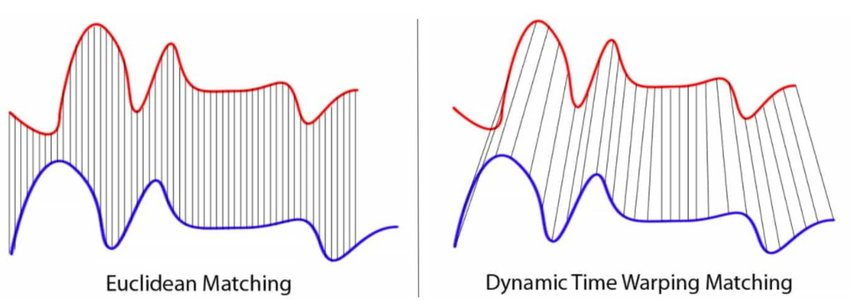
\includegraphics[scale=0.40]{slike/dtw1.png}
    \caption{Vizualna primerjava evklidske poravnave in poravnave z DTW}
\end{figure}

\section{Algoritem DTW}
Zapisa algoritma za izračun DTW razdalje se lotimo s konceptom dinamičnega programiranja. 
Primerjamo dve časovni vrsti $(a_i)_{i=1, \dots, m}$ in $(b_j)_{j=1, \dots, n}$ tako, da iščemo DTW razdaljo med njima: $D_{m,n}$. 
Ker se morata zadnja indeksa v vrstah ujemati ju bomo zagotovo poravnali in $D_{m,n}$ bo vsaj $d(a_m, b_n)$ (razdalja med njima). 
Naslednjo poravnamo lahko dobimo na 3 načine. Lahko poravnamo predzadnja indeksa obeh vrst, poravnamo zadnji indeks prve vrste in predzadnjega druge vrste ali obratno.
Če poravnamo predzadnja indeksa, je ta poravnava enaka zadnji poravnavi prvotnih vrst, ki jima odvzamemo zadnja indeksa. 
Ekvivalentno poravnava predzadnjega indeksa prve vrste z zadnjim indeksom druge vrste predstavlja zadnjo poravnavo, če prvi vrsti odvzamemo zadnji indeks.
Predpostavimo, da poznamo $D_{m-1,n-1}$, $D_{m-1,n}$, $D_{m,n-1}$. 
Potem je $D_{m,n} = d(a_m, b_n) + \min(D_{m-1,n-1}, D_{m-1,n}, D_{m,n-1})$, ker želimo izbrati poravnavo z najmanjšo ceno oz. DTW razdaljo.
Potem rekurzivno nadaljujemo in pridemo do robnih pogojev. Ker morata biti prva indeksa v vrsth poravnana bo $D_{1,1} = d(a_i, b_j)$. Če je prva vrsta dolžine $1$, potem ta 
indeks poravnamo z vsemi indeksi iz druge vrste in je $D_{1,n} = d(a_1, b_n) +  D_{m,n-1}$. Analogno velja, če je druga vrsta dolžine $1$.
\\
Spodaj zapisan algoritem, računa matriko cen poravnav, kjer število na $(i,j)$-tem mestu predstavlja DTW razdaljo, 
če poravnamo $(a_k)_{k=1, \dots, i}$ in $(b_l)_{l=1, \dots, j}$. Dodamo še ničta stolpec in vrstivo, da implementiramo robne pogoje.\\


\begin{algorithm}[H]
    \SetKwData{Left}{left}\SetKwData{This}{this}\SetKwData{Up}{up}
    \SetKwFunction{Union}{Union}\SetKwFunction{FindCompress}{FindCompress}
    \SetKwInOut{Input}{input}\SetKwInOut{Output}{output}

    \SetAlgoLined
    \Input{$(a_i)_{i=1, \dots, m}$ in $(b_j)_{j=1, \dots, n}$ \tcp*{časovni vrsti}} 
    \Output{$D_{m,n}$ \tcp*{DTW razdalja}} 
     \BlankLine
     $D \in \R^{(m+1)\times(n+1)}$\\ 
     \For{$i\leftarrow 1$ \KwTo $m$}{$D_{i,0} \leftarrow \infty$}
     \For{$j\leftarrow 1$ \KwTo $n$}{$D_{0,j} \leftarrow \infty$}
     $D_{0,0} \leftarrow 0$ \\
     \For{$i\leftarrow 1$ \KwTo $m$}{
        \For{$j\leftarrow 1$ \KwTo $n$}{
            $D_{i,j} \leftarrow d(a_i, b_j) + \min(D_{i-1,j-1}, D_{i-1,j}, D_{i,j-1})$
        }
     }
     \caption{DTW algoritem}
    \end{algorithm}

\section{Upraba DTW}
Algoritem se pogosto uprablja:
\begin{itemize}
    \item za obdelavo avdio podatkov. V avdio sistemih se uporablja za prepozavnje zvokov govora, ki lahko imajo različno hitrost govorenja.  
    \item v financah za ocenjevanje kvalitete napovednih modelov v primerjavi z resničnimi podatki. 
    \item iskanje delnic in indeksov s  podobnim gibanjem
\end{itemize}

\section{Uporaba razdalje DTW za grupiranje podatkov}
Za opazovane podatke sva si izbrala mesečni cenovni indeks delnic, ki 
kotirajo na domačih borzah. Podatki so za 21 držav evropske unije ter še 
indeks za evropsko unijo.

Najprej je bilo potrebno izračunati distančno matriko, to je spodnje trikotna matrika,
v kateri so izračunane DTW razdalje med vsemi indeksi posameznih držav.
Nato z vrgrajnimi funkcijami v \textbf{R} , kot je \emph{hclust()} izdelamo hirarični diagram
\\
Naši rezultati so naslednji:
\\

\begin{figure}[h!]
    \centering
    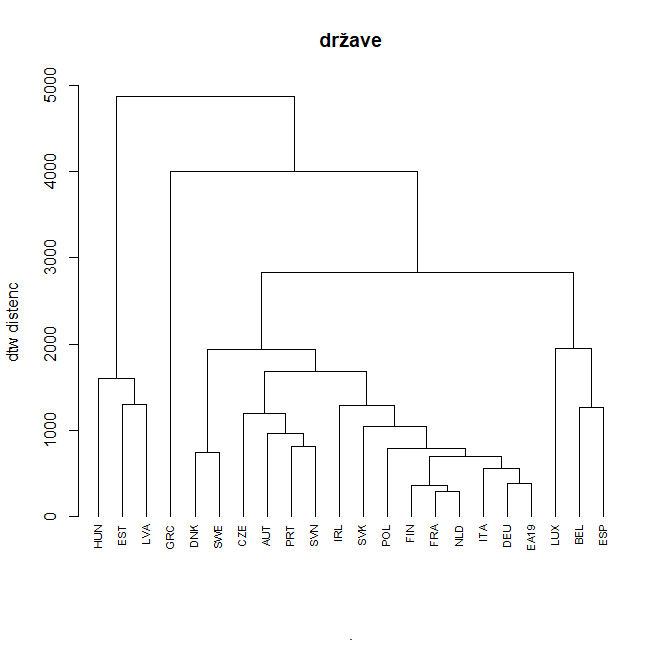
\includegraphics[scale=0.45]{slike/hirar.png}
    \caption{Hirarhični diagram}
\end{figure}

\subsection{Določitev optimalnega števila skupin}
Kot vemo je pri grupiranju podatkov problem določiti, v koliko skupin naj razvrstimo opazovane podatke.
Ena od preprostejših medtod, za določitev najbolj primernega števila skupin, je
kolenska metoda, ki deluje na principu, da računa razdaljo med skupinama, ki smo ju združili.
Za optimalno število skupin pa vzamemo tisto število skupin, pri katerem je bil padec v razdaljah, ko 
dodamo novo skupino, največji. V nalogi smo optimalno število določili računsko, lahko pa si pomagamo
tudi grafično in sicer tako, da iščemo točko z največjim padcem. \\
Poglejmo si graf za naše podatke:\\
\begin{figure}[h!]
    \centering
    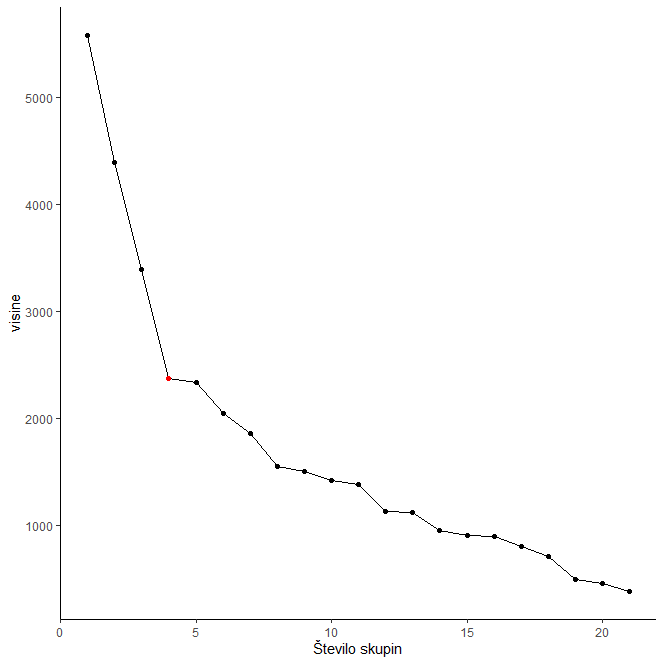
\includegraphics[width=1.0\linewidth,height=0.5\textheight]{slike/kolena.png}
    \caption{graf za iskanje optimalnega števila skupin}
\end{figure}

Za optimalno število skupin  smo tako določili število 4. Sedaj pa te 4 skupine 
narišimo še na naš hirarhični diagram\\
\begin{figure}[h!]
    \centering
    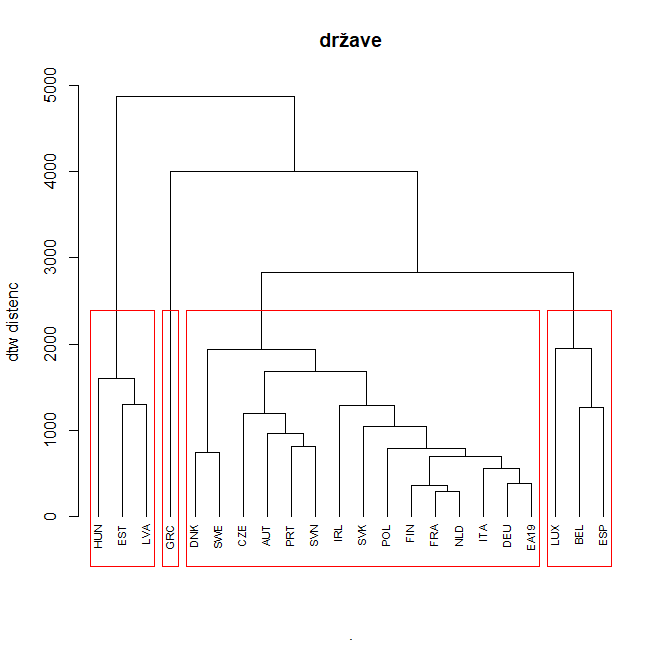
\includegraphics[scale=0.43]{slike/skupine.png}
    \caption{skupine na hirarhičnem diagramu}
\end{figure}

\pagebreak
Poglejmo si še razvrstitev v skupine na zemljevidu Evrope 
\begin{figure}[h!]
    \centering
    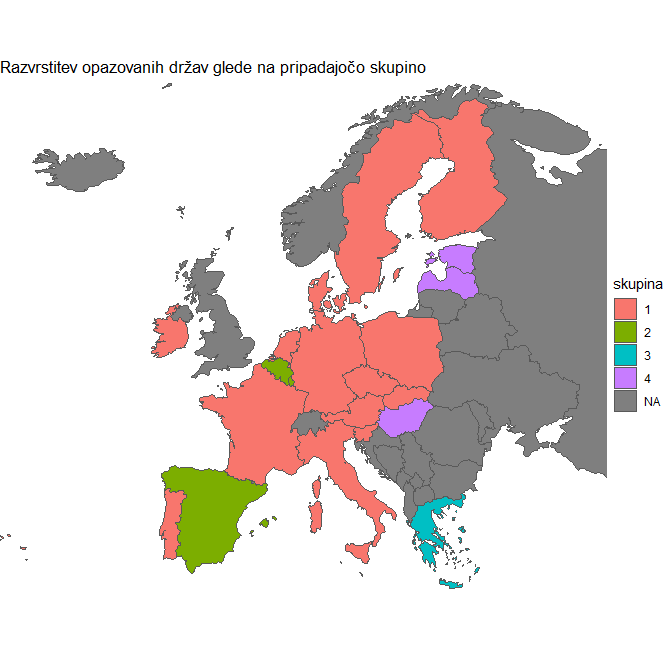
\includegraphics[scale=0.40]{slike/zemljevid.png}
    \caption{razvrstitev v skupine na zemljevidu}
\end{figure}

\section{Srednje vrednosti}
V splošnem je to širok pojem, rešitev le te pa je odvisna od tega, kako si problem zastavimo.
V splošni praksi največkrat iščemo povprečno vredost ali pa mediano, podobno stvar pa želimo prensti na 
časovne vrste.\\

\textbf{Povprečna časovna vrsta} bi bila neka nova časovna vrsta, ki minimizira vsoto DTW razdalj
do opazovanih časovnih vrst. V splošnem je iskanje take časovne vrste zelo zahtevn problem, zato ju v najini
nalogi ne bomo obravnavli.\\

\textbf{Medianska časovna vrsta} je tista časovna vrsta iz opazovanih časovnih vrst, katere vsota DTW razdalj
do ostalih časovni vrst je minimalna. Če prav se definicija na prvi pogled zdi zelo podobna definiciji
povprečne časovne vrste je glavna razlika v tem, da medianska časovna vrsta je ena izmed opazovanih časovnih vrst,
povprečna časovna vrsta pa je nova časovna vrsta,ki jo moremo
izračunati/določiti.\\

Matematično definicijo zapišemo takole:\\
\\
\emph{Naj bo $X=\{x_{1},x_{2},\dots,x_{n}\}$ možica časovnih vrst, medianska časovna vrsta $x_{Medi}$ iz možice $X$ je časovna vrsta za katero velja}
\begin{center}\[x_{Medi}=\min_{y \in X} \sum_{n=1}^{n} DTW(y,x_{i}) \]\end{center} 

Glede na to, da imamo že izračunano distančno  (privzamemo da je vsaka razdalja izračuna pod in nad diagonalo), je iz te določiti mediansko časovno vrsto precej enostavno, saj je vse, kar je
potrebno je to, da seštejemo vse stolpce ali vse vrstice, določimo minimalno vsoto in očitamo, pri kateri časovni vrsti je bil minimum dosežen.\\

V našem primeru je mediano dosegel indeks cen delnic na Nizozemskem. Zanimivo je tudi poiskati mediansko časovno vrsto za vsako skupino, ki smo jo 
dobili pri grupiranju. Pri velikem številu časovnih vrst in velikem številu skupin pri grupiranju je pogosta
praksa, da se pri izrisovanju podatkov izriše samo mediansko časovno vrsto v vsaki skupini,kot najbolj primernega prestavnika skupine.

\section{Izris podatkov}

Na naslednji sliki lahko vidimo izrisane naše opazovane indekse razvrščene po skupinah.
Z črtkano črto je označen medianski indeks v posamezni skupini.\\
\begin{figure}[h!]
    \centering
    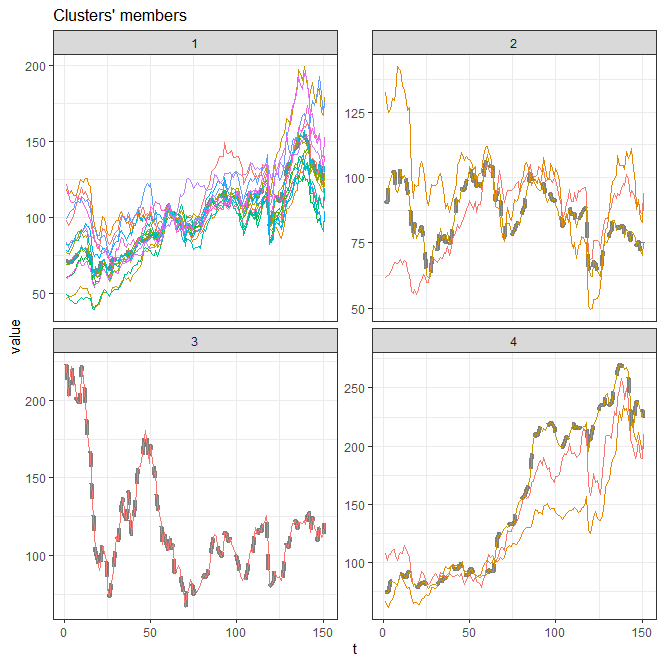
\includegraphics[scale=0.60]{slike/4_skupine.png}
    \caption{izris indeksov po skupinah}
\end{figure}

\pagebreak
Kot zanimivost dodajmo še izris indeksov če jih razvrstimo v 8 skupin

\begin{figure}[h!]
    \centering
    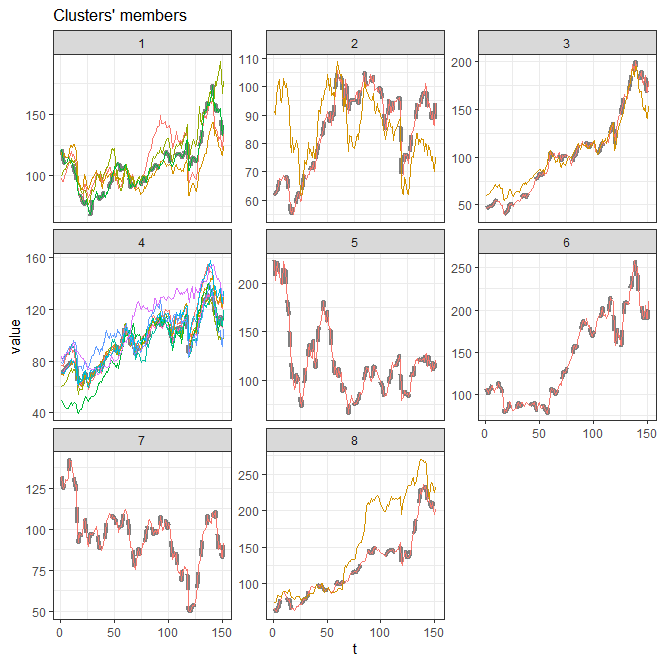
\includegraphics[scale=0.60]{slike/8_skupin.png}
    \caption{izris indeksov v 8 skupinah}
\end{figure}
\pagebreak
\section{Opombe}
Pri izračunu DTW razdalje z našim algoritmom ali pa z vgrajenim algoritmom iz \textbf{R}-ja je prihajalo do 
odstopanj vredosti, so pa vsi nadalni rezultati grupiranja in iskanje mediane, dali iste rezultate.
Po posvetovanju in pregledu algoritmov na konzultacijah, smo prišli do zaključov, da vgrajeni algoritem uporablja
nekoliko drugačno metodo.

\pagebreak

% seznam uporabljene literature
\begin{thebibliography}{99}

    \bibitem{dtw_vs_euc}
    Slika vizualne primerjave DTW in evklidske poravnave, [ogled 9.~1.~2023], dostopno na \url{https://www.researchgate.net/publication/350397933/figure/fig2/AS:1005448887025665@1616729103138/Simple-visualization-of-dynamic-time-warping-DTW-alignment-Instead-of-assuming-a.jpg}.
    
    \bibitem{wiki_DTW}
    \emph{Dynamic time warping}, v: Wikipedia: The Free Encyclopedia, [ogled 9.~1.~2023], dostopno na \url{https://en.wikipedia.org/wiki/Dynamic_time_warping}.

    \bibitem{DTW1}
    \emph{Introduction To Dynamic Time Warping}, [ogled 9.~1.~2023], dostopno na \url{https://riptutorial.com/algorithm/example/24981/introduction-to-dynamic-time-warping}.

    \bibitem{DTW2}
    \emph{lecture dtw notebook}, v: GitHub, [ogled 9.~1.~2023], dostopno na \url{https://github.com/kamperh/lecture_dtw_notebook/blob/main/dtw.ipynb}.

    \bibitem{clust1}
    \emph{Razvrščanje v skupine: Uvod}, [ogled 9.~1.~2023], dostopno na \url{https://kt.ijs.si/~ljupco/lectures/appr/09-razvrscanje-v-skupine-1.nb.html}.

    \bibitem{clust2}
    \emph{Razvrščanje v skupine: Vrednotenje kvalitete razvrščanja}, [ogled 9.~1.~2023], dostopno na \url{https://kt.ijs.si/~ljupco/lectures/appr/10-razvrscanje-v-skupine-2.nb.html}.

    \bibitem{DTW3}
    \emph{An introduction to Dynamic Time Warping}, [ogled 9.~1.~2023], dostopno na \url{https://rtavenar.github.io/blog/dtw.html}.

    \bibitem{clust3}
    \emph{Dynamic Time Warping (DTW) as a mean to cluster time series}, [ogled 9.~1.~2023], dostopno na \url{https://rpubs.com/esobolewska/dtw-time-series}.

    \bibitem{clust4}
    \emph{Generalized k-means-based clustering for temporal data under time warp}, [ogled 9.~1.~2023], dostopno na \url{https://theses.hal.science/tel-01680370/document}.

\end{thebibliography}

\end{document}

